\setAuthor{Valter Kiisk}
\setRound{lõppvoor}
\setYear{2007}
\setNumber{G 3}
\setDifficulty{2}
\setTopic{Geomeetriline optika}

\prob{Kiil}
Laserkiire teele asetatakse enam-vähem risti õhuke klaasplaat (klaasi murdumisnäitaja $n = \num{1,5}$). Selle tulemusena nihkub $L = \SI{2}{m}$ kaugusel ekraanil olev laserkiire kujutis $d = \SI{5}{mm}$ võrra. Järeldatakse, et plaat on kergelt kiilukujuline. Leidke selle kiilu tipunurk $\alpha$. 

\emph{Vihje:} väikeste nurkade $\varphi$ puhul $\sin \varphi \approx \tan \varphi \approx \varphi$.

\hint
Laserkiire kõrvalekaldenurk on leitav Snelli seaduse ja kiilu geomeetria rakendamisest.

\solu
Kõik nurgad on tähistatud järgneval joonisel. $\alpha$ on meelevaldne (kuigi $\alpha \ll 1$). $\beta = \alpha /n$. $\gamma = \beta - \epsilon$. $\delta = n\gamma = \alpha - n\epsilon$. Kiire kõrvalekaldenurk
\[
\phi=(\alpha-\beta)-(\delta-\gamma)=(\alpha-\delta)+(\gamma-\beta)=n \epsilon-\epsilon=\epsilon(n-1).
\]
Teades, et $\phi = \SI{5}{mm}/\SI{2}{m} = \SI{0.0025}{rad}$, saame
\[
\epsilon=\frac{\phi}{n-1}=\SI{0,005}{rad}=\ang{0,29}.
\]

\begin{center}
	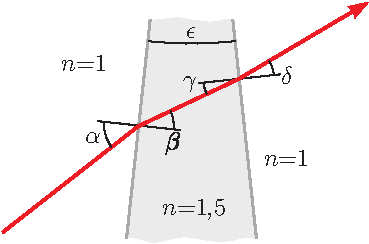
\includegraphics[width=0.7\textwidth]{2007-v3g-03-yl}
\end{center}
\probend